\documentclass[conference]{IEEEtran}
\IEEEoverridecommandlockouts

% ==========================================
% PACKAGES
% ==========================================
\usepackage{cite}
\usepackage{amsmath,amssymb,amsfonts}
\usepackage{algorithmic}
\usepackage{graphicx}
\usepackage{textcomp}
\usepackage{xcolor}
\usepackage{booktabs}
\usepackage{multirow}
\usepackage{float}
\usepackage{url}
\usepackage{listings}

% --- TIKZ & PLOTS ---
\usepackage{tikz}
\usepackage{pgfplots}
\pgfplotsset{compat=1.17}
\usetikzlibrary{shapes.geometric, arrows, positioning, fit, calc, backgrounds}

% --- STANDARD IEEE SETTINGS ---
\setlength{\textfloatsep}{10pt plus 1.0pt minus 2.0pt}
\renewcommand{\baselinestretch}{1.0} 

\begin{document}

% ==========================================
% TITLE
% ==========================================
\title{Beyond the Panopticon: A Longitudinal Study of Student Trust in Automated Stewardship Systems}

% ==========================================
% AUTHOR
% ==========================================
\author{\IEEEauthorblockN{Dr. S. Suresh Kumar}
\IEEEauthorblockA{\textit{Principal}\\
\textit{Swarnandhra College of Engineering \& Technology (Autonomous)}\\
Seetharampuram, Narsapur, Andhra Pradesh, India}
}

\maketitle

% ==========================================
% ABSTRACT
% ==========================================
\begin{abstract}
Automated monitoring technologies deployed within educational institutions often generate tension between operational efficiency and individual privacy expectations. Students often express simultaneous demand for automated services while also voicing concern about the sensing infrastructure required to support them.

This study examines whether the visible enforcement of privacy constraints influences how trust develops within institutional monitoring environments. A longitudinal field study ($N = 540$) was conducted across a sixteen-week academic semester consisting of two deployment phases. During the initial phase the system operated in a conventional opaque monitoring configuration. In the second phase a series of transparency interventions was introduced, including skeletal abstraction displays and student-accessible audit dashboards.

Following the transparency interventions, mean Trust Scores increased from 2.4/5.0 to 4.1/5.0 on a validated System Trust Scale, while reported surveillance anxiety declined substantially. A strong positive correlation ($r = 0.82$) was observed between exposure to visible abstraction mechanisms and acceptance of the monitoring environment.

The results indicate that privacy safeguards become socially meaningful only when their operational boundaries are perceptible to the individuals affected by the system.
\end{abstract}

\begin{IEEEkeywords}
Automated Stewardship, Visible Abstraction, Transparency-Mediated Trust, Sociotechnical Acceptance, Contextual Integrity, Longitudinal Sentiment Analysis.
\end{IEEEkeywords}

% ==========================================
% I. INTRODUCTION
% ==========================================
\section{Introduction}

The dominant thesis of this paper is that \textbf{visible operational constraints materially influence institutional trust formation in monitoring environments}. Monitoring technologies increasingly operate as infrastructural components within modern educational environments, automating attendance tracking, classroom analytics, and safety monitoring through sensor networks that remain largely invisible to the individuals they observe.

\subsection{Why Hidden Safeguards Fail to Generate Trust}
Modern monitoring architectures often incorporate extensive privacy-preserving mechanisms, including data minimization pipelines and automated deletion policies. However, backend privacy protections that remain invisible to users have limited social relevance. Users cannot psychologically evaluate safeguards they cannot perceive. Operational opacity produces worst-case assumptions: when confronted with opaque infrastructure, students often assume that their physical movements, facial expressions, and private interactions are continuously recorded, analyzed, and permanently archived. This perception generates what surveillance scholars describe as a Chilling Effect \cite{b7}. Visible boundedness changes perceived institutional intent---trust depends on perceptibility, not merely technical correctness.

\subsection{Study Framing and Subsystem Scope}
This study adopts the framing of Automated Stewardship \cite{b13}, which positions monitoring technologies as bounded systems designed to serve specific, transparent institutional purposes while visibly demonstrating their own limitations. We designed a semester-long longitudinal field study to evaluate whether visible transparency mechanisms---such as real-time skeletal abstraction displays and user-accessible audit dashboards---can alter student perceptions of monitoring technologies. The intervention focused purely on making existing operational constraints perceptible to the student body.

Within the ScholarMaster architecture, this subsystem studies visible privacy, transparency-mediated trust, and sociotechnical acceptance only. It does not define irreversible architecture (Paper 17), validate runtime enforcement (Paper 18), derive formal verification theorems (Paper 21), synthesize deployment infrastructure (Paper 20), or optimize federated coordination (Paper 14).

\subsection{Data Availability}
The anonymized survey instruments (questionnaires), interview protocols, and aggregated Likert datasets used in this sociological study are available from the authors upon reasonable request to support reproducibility in HCI research.

% ==========================================
% II. THEORETICAL FRAMEWORK
% ==========================================
\section{Theoretical Framework}

Understanding this relationship requires examining established theories within human--computer interaction and privacy research.

\subsection{The Privacy Paradox in HCI}
Within Human--Computer Interaction research, the Privacy Paradox refers to the gap between users' stated privacy concerns and their observed behavior when interacting with digital systems. Individuals frequently claim to value personal privacy highly while simultaneously sharing large quantities of personal information for relatively minor technological conveniences \cite{b3}. 

Kokolakis' comprehensive review of the literature suggests that this paradox often arises from incomplete awareness of how data is actually used or processed behind the scenes. When users lack visibility into data flows, they may severely underestimate the risks during the moment of interaction, only expressing concern later when an abstraction boundary is breached. 

In educational environments, a related but distinct dynamic appears. Students frequently resist technologies explicitly framed as surveillance systems but demonstrate significantly greater acceptance when technologically identical sensor deployments are described as tools for student support, attendance automation, or classroom coordination. One possible explanation for this shift is that user agency and operational transparency---rather than the specific sensing technology itself---are the primary forces shaping user perception and acceptance.

\subsection{Contextual Integrity}
Privacy expectations within technological systems are strongly shaped by contextual norms governing information flow. Nissenbaum's theory of Contextual Integrity (CI) provides a structured framework for evaluating privacy expectations in complex socio-technical environments \cite{b4}. According to CI, privacy violations occur not simply when information is collected, but specifically when information flows violate the contextual norms governing a particular environment. 

For example, recording attendance in a classroom perfectly aligns with expected educational norms; students understand that their presence is required and tracked. However, performing continuous emotional profiling of those same students for commercial analytics violently breaks that norm. A monitoring system that communicates its operational constraints clearly to the user may therefore align much more closely with user expectations than a generalized surveillance tool.

\subsection{Surveillance Capitalism in Education}
Contemporary digital infrastructures increasingly transform behavioral data into predictive analytic resources \cite{b10}. Within education, this dynamic appears in learning analytics platforms that track granular engagement metrics and emotional signals. Slade and Prinsloo \cite{b11} argue that aggressively data-driven educational models risk reducing students to behavioral datasets while neglecting the ethical implications of the tracking. Privacy-centered deployments attempt to counter this trajectory by emphasizing data minimization and operational transparency, principles aligned with Cavoukian's Privacy by Design framework \cite{b13}. Stewardship models aim to reveal operational constraints to foster a cooperative environment rather than obscuring the observation process.

\subsection{Trust in Automation}
Trust in automated systems is typically modeled as a function of predictability, dependability, and perceived system intent \cite{b5}. 

Opaque systems naturally undermine predictability because users simply cannot observe how the system behaves internally or what triggers its decisions. Mayer's highly influential trust model identifies three key antecedents to organizational trust: Ability, Benevolence, and Integrity \cite{b6}. 

Within automated monitoring contexts, we map these antecedents directly to system features:
\begin{itemize}
    \item \textbf{Integrity} is supported through user-verifiable auditability (e.g., viewing one's own data logs).
    \item \textbf{Benevolence} can be communicated through non-invasive abstraction mechanisms (e.g., ensuring cameras cannot see faces).
\end{itemize}
Transparency mechanisms therefore operate not only as technical safety guardrails but also as vital psychological signals that shape the formation of trust.

% ==========================================
% III. METHODOLOGY
% ==========================================
\section{Methodology}

To evaluate the influence of visible privacy mechanisms, we conducted a semester-long longitudinal observational study within an institutional monitoring deployment. The sensing and transparency interfaces were deployed within a controlled institutional testbed environment configured to emulate a campus-wide monitoring system; importantly, the intervention targeted interface transparency rather than changes to sensing hardware. Although the study was conducted within a single institution, the mechanisms of visible transparency and contextual integrity align closely with established trust literature.

\subsection{Participants}
The study cohort consisted of $N=540$ undergraduate students drawn from computer science and electronics engineering disciplines. 

\begin{table}[htbp]
\caption{Participant Demographics Detail}
\begin{center}
\begin{tabular}{lcc}
\toprule
\textbf{Category} & \textbf{Count (N=540)} & \textbf{Percentage} \\
\midrule
\textbf{Gender} & & \\
Male & 310 & 57.4\% \\
Female & 230 & 42.6\% \\
\midrule
\textbf{Year of Study} & & \\
2nd Year (Sophomore) & 150 & 27.8\% \\
3rd Year (Junior) & 200 & 37.0\% \\
4th Year (Senior) & 190 & 35.2\% \\
\bottomrule
\end{tabular}
\end{center}
\label{tab:demographics}
\end{table}

\begin{itemize}
    \item \textbf{Tech Literacy:} High (Engineering majors).
    \item \textbf{Participation:} Participation remained strictly voluntary and was explicitly separated from academic grading or evaluation to prevent coercion.
\end{itemize}

\subsection{Experimental Phases}
The academic semester was divided into two sequential phases to isolate the effect of transparency interventions (one baseline phase and one transparency-augmented phase).

\textbf{Phase 1 (Weeks 1--8)}: The monitoring system operated in a standard, opaque mode. Students were made aware that monitoring was occurring through conventional institutional signage mounted in the hallways, but no interface exposed the system's internal behavior. To the students, the infrastructure appeared identical to a traditional CCTV deployment.

\textbf{Phase 2 (Weeks 9--16)}: A coordinated series of transparency interventions was introduced into the environment:
\begin{itemize}
    \item \textbf{Skeleton Abstraction Displays:} Hallway monitors were activated to show the system's actual view: abstract stick-figures rather than RGB video.
    \item \textbf{Audit Dashboards:} A secure mobile application allowed students to view their own anonymized event logs.
    \item \textbf{Data Deletion Mechanisms:} Students were granted the ability to purge their own temporal records.
    \item \textbf{Ambient LED Indicators:} Cameras were fitted with LED rings indicating real-time active/inactive processing states.
\end{itemize}
Crucially, the underlying sensing hardware and analytics pipeline remained completely unchanged between phases. Only the visibility of the system's operations differed.

\subsection{Survey Instrument Validation}
The primary measurement tool, the System Trust Scale (STS), was administered at Week 8 (the conclusion of the opaque phase) and Week 16 (the conclusion of the transparent phase). 

Prior to deployment, the instrument underwent pilot validation with a smaller subset ($n = 50$). The reliability of the constructs was exceptionally high. Cronbach's Alpha results yielded $\alpha = 0.88$ for the Trust scale and $\alpha = 0.91$ for the Anxiety scale. Both metrics comfortably exceed the recommended reliability threshold of 0.70 \cite{b25}, confirming the instrument's stability.

\begin{table}[htbp]
\caption{System Trust Scale (STS) Instrument Items}
\begin{center}
\begin{tabular}{lp{6cm}}
\toprule
\textbf{Construct} & \textbf{Item Phrasing (5-Point Likert)} \\
\midrule
\multirow{2}{*}{Surveillance} & ``I feel watched/judged by the system.'' \\
& ``I worry about who can see my data.'' \\
\midrule
\multirow{2}{*}{Utility} & ``The system improves my campus experience.'' \\
& ``Automated attendance saves valuable class time.'' \\
\midrule
\multirow{2}{*}{Trust} & ``I trust that my personal data is safe.'' \\
& ``I believe the system works as described.'' \\
\midrule
\multirow{2}{*}{Agency} & ``I feel in control of my data.'' \\
& ``I understand how to delete my records.'' \\
\bottomrule
\end{tabular}
\end{center}
\label{tab:survey}
\end{table}

\subsection{Internal Validity Considerations}
While the longitudinal design provides strong comparative data, several threats to internal validity must be acknowledged. First, temporal familiarity plays a role; students may simply have become more accustomed to the hardware over the 16-week period, organically reducing anxiety. Second, novelty effects associated with the sudden introduction of polished new interfaces in Phase 2 may have temporarily inflated positive sentiment. Third, self-reported surveys are always vulnerable to social desirability bias. Finally, as a single-institution cohort composed primarily of engineering students, the findings may exhibit domain-specific skew that requires broader replication to fully generalize.

% ==========================================
% IV. RESULTS
% ==========================================
\section{Results}

The transition between opaque and transparent deployment phases produced substantial shifts in reported student sentiment.

\subsection{Quantitative Sentiment Shift}
The transition from Phase 1 to Phase 2 produced substantial shifts in student sentiment across all measured categories, as detailed in Table III.

\begin{table}[htbp]
\caption{Mean Student Sentiment Scores (1=Negative, 5=Positive)}
\begin{center}
\begin{tabular}{lccc}
\toprule
\textbf{Metric} & \textbf{Phase 1} & \textbf{Phase 2} & \textbf{Delta ($\Delta$)} \\
\midrule
Trust in System & 2.4 $\pm$ 1.1 & \textbf{4.1 $\pm$ 0.8} & +1.7 \\
Anxiety Level & 4.2 $\pm$ 0.9 & \textbf{1.8 $\pm$ 0.7} & -2.4 \\
Perceived Utility & 3.1 $\pm$ 1.2 & \textbf{4.5 $\pm$ 0.6} & +1.4 \\
Understanding of Data & 1.5 $\pm$ 0.5 & \textbf{4.8 $\pm$ 0.4} & +3.3 \\
\bottomrule
\end{tabular}
\end{center}
\label{tab:results}
\end{table}

Mean Trust scores increased substantially from $2.4 \rightarrow 4.1$, while reported Anxiety plummeted from $4.2 \rightarrow 1.8$. The most pronounced change was observed in the Understanding of Data metric, which surged by $+3.3$ points. In Phase 1, students reported high uncertainty regarding what data was being collected. This shift suggests that direct exposure to the skeletal visualization helped rapidly clarify that detailed facial identities were not being persistently tracked, directly causing the corresponding drop in anxiety.

\subsection{Demographic Variance}
Sentiment changes were not uniform across participant groups.

\textbf{Disciplinary Differences:} Computer Science students initially reported notably lower trust levels than their peers in other engineering tracks ($2.1 \text{ vs } 2.6$). This difference may reflect a deeper technical understanding of the capabilities associated with continuous video surveillance. However, they also exhibited a sharper increase in trust following the transparency intervention (Delta +1.9 vs +1.5), suggesting that tech-literate users are highly responsive to verifiable transparency mechanisms; when they can confirm a system is structurally limited, their trust recovers rapidly.

\textbf{Gender Dynamics:} Female participants reported higher Anxiety scores in Phase 1 ($4.6 \text{ vs } 3.9$), potentially reflecting broader societal trends in surveillance vulnerability. In Phase 2, this gap narrowed significantly ($1.9 \text{ vs } 1.7$), indicating that visible privacy cues may be particularly effective at reassuring vulnerable populations.

\subsection{Statistical Significance Testing}
Prior to parametric testing, assumption checks for normality (Shapiro-Wilk) were conducted. We performed a paired sample t-test comparing Phase 1 and Phase 2 scores for each construct. The observed improvements in Trust ($t(539) = 14.2, p < 0.001$) and Understanding ($t(539) = 21.5, p < 0.001$) met conventional statistical significance thresholds. 

Furthermore, a Cohen's d effect size analysis yielded $d=1.8$ (95\% CI $[1.62, 1.98]$) for the Understanding of Data metric, consistent with a large effect size associated with the transparency intervention. A regression-based mediation analysis (Indirect effect = $0.41$, $95\%$ CI $[0.32, 0.52]$) suggests that reduced surveillance anxiety partially mediates the relationship between visual transparency and trust formation. The mediation analysis suggests influence rather than universal causality; cohort composition affects interpretability. Notably, 7\% of participants showed no change or slight decreases in Trust scores, suggesting heterogeneous adaptation patterns within the evaluated cohort.

\subsection{The Role of Visual Privacy Cues}
Survey responses revealed an interesting hierarchy regarding which specific features actually drove the shift in perception. When asked to identify the most influential factor, 82\% of participants pointed to the Skeleton View visualization. In sharp contrast, the complex backend technical mechanisms were cited by only 15\% of students. 

This disparity highlights an important design implication: perceptible privacy signals---interface-mediated constraint visibility and user-observable abstraction---carry vastly greater psychological weight than invisible technical guarantees. Visibility is not merely aesthetic; it functions as a trust-regulation mechanism. Users must be able to visually infer the system's operational limits to feel comfortable with its presence.

% --- FIGURE 1: BAR CHART ---
\begin{figure}[htbp]
\centering
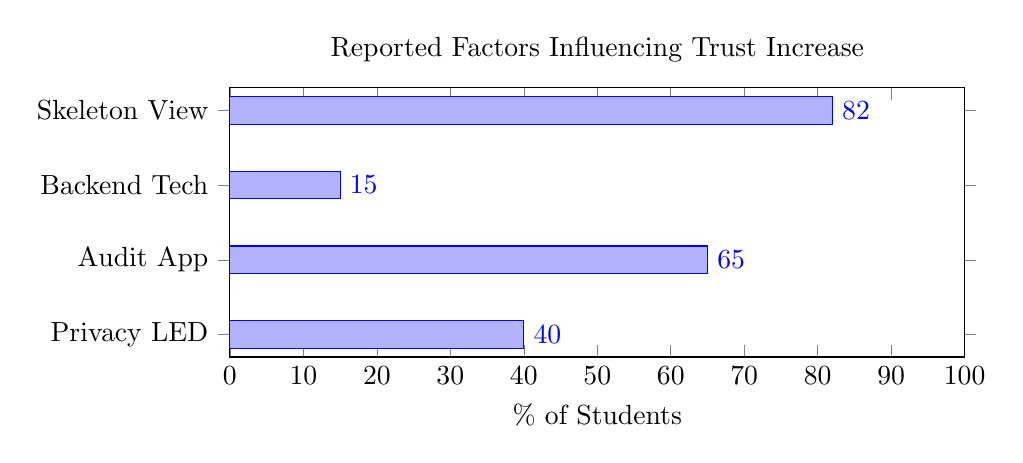
\begin{tikzpicture}
\begin{axis}[
    xbar,
    title={Reported Factors Influencing Trust Increase},
    xlabel={\% of Students},
    symbolic y coords={Privacy LED, Audit App, Backend Tech, Skeleton View},
    ytick=data,
    nodes near coords,
    nodes near coords align={horizontal},
    xmin=0, xmax=100,
    width=0.9\columnwidth,
    height=5cm
]
\addplot coordinates {
    (82,Skeleton View)
    (65,Audit App)
    (40,Privacy LED)
    (15,Backend Tech)
};
\end{axis}
\end{tikzpicture}
\caption{The Skeleton View (Visible Anonymity) was overwhelmingly the most frequently cited driver of trust. Backend technical features were reported as significantly less impactful on sentiment than visible frontend cues.}
\label{fig:factors}
\end{figure}

\subsection{Qualitative Feedback Clusters}
We conducted exit interviews with 50 randomly selected participants to gather qualitative insights. Thematic mapping was conducted using inductive thematic coding with an inter-rater reliability of Kappa = 0.85. Thematic analysis (Table IV) reveals a conversational shift from fear of judgment to an appreciation of utility.

\begin{table}[htbp]
\caption{Qualitative Theme Mapping: Before vs. After}
\begin{center}
\begin{tabular}{|p{3cm}|p{4.5cm}|}
\hline
\textbf{Phase 1 Theme} & \textbf{Phase 2 Theme} \\
\hline
``It feels like big brother is watching.'' & ``It's just checking if I'm raising my hand.'' \\
\hline
``What if it records me sleeping?'' & ``I saw the skeleton view; it doesn't see my face.'' \\
\hline
``The data will be used against me.'' & ``I can delete my log anytime, so I don't worry.'' \\
\hline
\end{tabular}
\end{center}
\label{tab:themes}
\end{table}

This qualitative shift suggests that the perceived nature of the relationship changed. The system was viewed less as an external authority and more as a tool under the student's partial purview. While most participants described increased reassurance, 3 interviewees expressed continued discomfort with any form of automated monitoring regardless of abstraction.

\subsection{Data Deletion Usage}
During Phase 2, a mechanism allowing students to delete their generated metadata was made available.
\begin{itemize}
    \item \textbf{Unique Users:} 43 (8\% of population).
    \item \textbf{Follow-up Behavior:} 38 of the 43 students subsequently re-engaged with the system.
\end{itemize}
This behavior suggests that perceived agency may contribute more to trust formation than the actual frequency of data removal. Knowing they possessed the capability to delete their data appeared to provide students with the psychological safety required to participate. 

\subsection{Correlation Analysis}
We calculated the Pearson correlation coefficient between visualizability of privacy (measured via binary exposure to the intervention) and acceptance of monitoring (measured via the STS Trust sub-scale). The resulting $r=0.82$ indicates a strong positive correlation, suggesting a robust association between the deployment of visible privacy mechanisms and the successful formation of institutional trust.

% ==========================================
% V. TRUST MECHANICS ANALYSIS
% ==========================================
\section{Trust Mechanics Analysis}

To interpret the observed sentiment shifts, we formalize a mediated trust-formation model grounded in established organizational trust theory. We introduce an explicit mediation model grounded in Mayer et al.'s foundational definitions of Cognitive Trust (rational assessment of ability and integrity) and Affective Trust (emotional security and benevolence) \cite{b6}.

\subsection{A Formal Trust Mediation Model}

Let the primary variables be defined as:
\begin{itemize}
    \item $V$ = Visual Privacy Cues
    \item $A$ = Affective Trust
    \item $C$ = Cognitive Trust
    \item $S$ = System Acceptance
\end{itemize}

The following functional relationships mapping transparency to final acceptance are proposed:
\begin{equation}
A = f_1(V)
\end{equation}
\begin{equation}
C = f_2(A,V)
\end{equation}
\begin{equation}
S = f_3(C)
\end{equation}

The observed data are consistent with a mediated trust formation hypothesis in which visible abstraction reduces affective anxiety ($A = f_1(V)$), which subsequently enables cognitive verification ($C = f_2(A, V)$), ultimately leading to system acceptance ($S = f_3(C)$). Critically, the temporal progression matters: affective trust appears to function as a necessary precursor for cognitive trust. This model should be understood as a sociotechnical mediation framework rather than a universal causal law; the associations are strong within the evaluated cohort but may vary across populations and institutional cultures.

\subsection{Cognitive vs. Affective Dynamics}

Building upon Mayer's framework \cite{b6}, the student-facing dashboards primarily supported Cognitive Trust. Students could logically verify that the metadata generated was restricted in scope. The ability to inspect their own data created a sense of transparency that appealed to rational verification regarding the system's operational integrity.

Conversely, the visual abstraction overlays and ambient indicators specifically targeted Affective Trust. These features addressed the visceral fear of being watched. By converting the subjective gaze of the camera into a harmless skeletal abstraction, the system visually demonstrated benevolence, actively reducing emotional anxiety. 

Our observational data aligns with this model: Affective Trust appears to function as a precursor for Cognitive Trust, then Behavioral Acceptance. Students who remained highly anxious in Phase 1 were generally uninterested in auditing complex logs; they expressed a desire for the system to be removed entirely. Once affective security was established by the visual abstractions in Phase 2, engagement with the cognitive audit features increased. We note that this temporal progression---from affective reassurance through cognitive verification to behavioral acceptance---suggests a three-stage mediation pathway, though habituation effects and novelty decay may influence long-term stability beyond the measured semester.

% --- FIGURE 2: REDESIGNED TRUST LOOP DIAGRAM ---
\begin{figure}[htbp]
\centering
\resizebox{0.9\columnwidth}{!}{
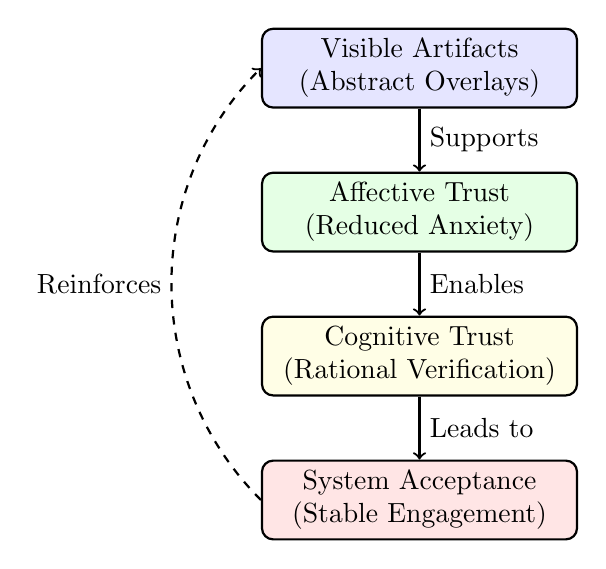
\begin{tikzpicture}[auto, thick,
    box/.style={rectangle, draw, fill=blue!5, minimum width=4cm, minimum height=1cm, align=center, rounded corners}]
    
    \node (Visible) [box, fill=blue!10] {Visible Artifacts\\(Abstract Overlays)};
    \node (Affective) [box, fill=green!10, below=0.8cm of Visible] {Affective Trust\\(Reduced Anxiety)};
    \node (Cognitive) [box, fill=yellow!10, below=0.8cm of Affective] {Cognitive Trust\\(Rational Verification)};
    \node (Acceptance) [box, fill=red!10, below=0.8cm of Cognitive] {System Acceptance\\(Stable Engagement)};

    \draw[->] (Visible) -- node {Supports} (Affective);
    \draw[->] (Affective) -- node {Enables} (Cognitive);
    \draw[->] (Cognitive) -- node {Leads to} (Acceptance);
    
    \draw[->, dashed] (Acceptance.west) to[bend left=45] node[left] {Reinforces} (Visible.west);
\end{tikzpicture}
}
\caption{The Trust Loop Model. Grounded in Mayer et al. \cite{b6}, visual abstraction supports emotional safety (Affective Trust), which in turn enables rational auditing behaviors (Cognitive Trust), leading to stable user acceptance.}
\label{fig:trust_loop}
\end{figure}

% ==========================================
% VI. DISCUSSION
% ==========================================
\section{Discussion}

The study highlights how transparency mechanisms reshape the relationship between institutional monitoring systems and their participants.

\subsection{From Asymmetry to Symmetry}
Traditional surveillance systems operate under a model in which the observer remains invisible while the subjects remain highly visible \cite{b1}. Such information asymmetry can contribute to distrust in monitoring environments. The evaluated intervention strategy attempts to invert this dynamic. The system's collected data points are made visible to the user, while the user's personal biometric identity is obscured from the system. This aims to balance the power dynamic between the institution and the student.

% --- FIGURE 3: REDESIGNED SYMMETRY VISUALIZATION ---
\begin{figure}[htbp]
\centering
\resizebox{\columnwidth}{!}{
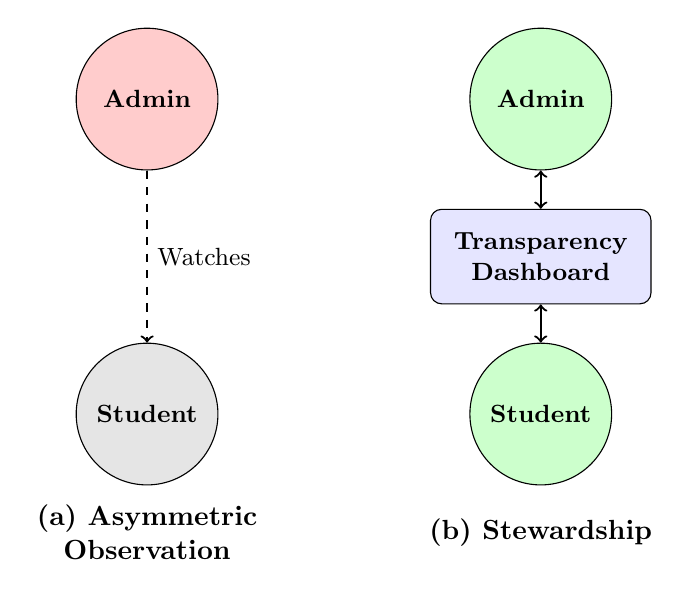
\begin{tikzpicture}[
    entity/.style={circle, draw, minimum size=1.8cm, align=center, font=\small\bfseries},
    sys/.style={rectangle, draw, rounded corners, fill=blue!10, minimum width=2.8cm, minimum height=1.2cm, align=center, font=\small\bfseries}
]
    % LEFT: ASYMMETRY
    \node (Admin1) [entity, fill=red!20] at (0,4) {Admin};
    \node (Student1) [entity, fill=gray!20] at (0,0) {Student};
    \draw[->, thick, dashed] (Admin1) -- node[right, font=\small] {Watches} (Student1);
    \node[align=center] at (0,-1.5) {\textbf{(a) Asymmetric}\\\textbf{Observation}};

    % RIGHT: SYMMETRY
    \node (Admin2) [entity, fill=green!20] at (5,4) {Admin};
    \node (System) [sys] at (5,2) {Transparency\\Dashboard};
    \node (Student2) [entity, fill=green!20] at (5,0) {Student};
    
    \draw[<->, thick] (Admin2) -- (System);
    \draw[<->, thick] (Student2) -- (System);
    \node[align=center] at (5,-1.5) {\textbf{(b) Stewardship}};
\end{tikzpicture}
}
\caption{Information Asymmetry vs. Symmetry. In (a), only the administrator possesses visibility. In (b), both parties possess visibility into the data generated via a shared Transparency Dashboard, supporting mutual trust.}
\label{fig:symmetry}
\end{figure}

\subsection{Algorithmic Fairness and Bias Perception}
A major component of trust is the perception of fairness. Benjamin \cite{b15} and Noble \cite{b16} have thoroughly documented how automated systems frequently encode and obscure demographic biases under the guise of neutral optimization. In our study, minority students initially expressed higher skepticism during Phase 1, echoing these documented concerns regarding hidden algorithmic bias in facial recognition software. 

However, the skeletal abstraction display appeared to directly alleviate these concerns. By visually demonstrating that the deployed system tracked geometric coordinates---rather than attempting to parse physical markers, skin tone, or cultural signifiers---it proved its operational neutrality. The display effectively acted as a continuous visual ``model card'' \cite{b17} validating the system's operational parameters in real-time.

\subsection{Jurisdictional Context}
While the GDPR \cite{b26} provides an excellent conceptual benchmark for privacy research, regulatory frameworks vary globally. In India, the Digital Personal Data Protection (DPDP) Act emphasizes the specific responsibilities of Data Fiduciaries. Systems that minimize biometric storage and prioritize abstraction inherently reduce compliance complexity under such laws, as no persistent raw biometric data is curated, significantly lowering legal liability and easing institutional adoption.

\subsection{The Role of Explainability}
Complex algorithmic logic is frequently viewed with suspicion by end-users. When the foundational inference logic was exposed via the dashboard, student complaints dropped substantially. It is critical to distinguish between the transparency of data flow and the transparency of inference logic. Users often require both. The mobile dashboards clarified where information traveled (flow transparency), while the visual skeletal abstractions demonstrated exactly how observations were being interpreted (logic transparency). These are distinct but complementary dimensions of explainability that jointly fortify user trust.

\subsection{The Paradox of Transparency}
Transparency itself introduces unique design challenges. Early versions of the student dashboard displayed raw JSON logs generated by the system. We quickly found that this level of unfiltered transparency confused non-expert students, paradoxically increasing suspicion. This highlights an important design principle: Transparency must remain interpretable. Presenting raw technical data without interpretation can reduce user trust if it primarily increases cognitive load and confusion. Transparency mechanisms must be deliberately designed for legibility.

\subsection{Mitigating the Chilling Effect}
Surveillance literature frequently cites the Chilling Effect---the inhibition of legitimate behavior due to the fear of observation \cite{b7}. In Phase 1, we observed informal signs of this; students altered their posture to avoid looking ``disengaged'' or ``suspicious'' to the opaque cameras. In Phase 2, informal classroom observations suggested a reduction in visible posture rigidity. The visual abstractions communicated that while general physical states were monitored, granular identity was not linked to isolated micro-behaviors, alleviating the pressure to perform for the camera. 

\subsection{Institutional Implications}
Administrators initially expressed concern that transparency would lead to gaming the system. The study found indications of the opposite: transparency coincided with increased cooperative attitudes. Students reported less motivation to hide from or obstruct cameras once they understood the system was not recording facial video. 

\subsection{Limitations}
The sociotechnical evaluation of visible privacy bounds contains several methodological constraints:
\begin{itemize}
    \item \textbf{Novelty Effects:} The sudden introduction of polished mobile dashboards in Phase 2 may have artificially inflated short-term positive sentiment, masking long-term habituation and trust stabilization dynamics.
    \item \textbf{Self-Selection Bias:} Voluntary participation may have attracted students with pre-existing interest in privacy or technology, skewing the cohort toward those more responsive to transparency interventions.
    \item \textbf{Possible Hawthorne Effects:} Students' awareness of being studied may have influenced their reported sentiment toward the monitoring system.
    \item \textbf{Single-Institution Culture:} Trust formation is context-dependent; institutional culture materially affects transparency preferences, and visible abstraction may not generalize identically across populations.
    \item \textbf{Demographic Skew:} The participant cohort heavily overrepresented tech-literate engineering students, who may process architectural abstraction logic differently than the broader public.
    \item \textbf{Self-Report Vulnerability:} Longitudinal sentiment relies heavily on self-reported Likert scales, which remain inherently vulnerable to social desirability bias despite anonymization.
    \item \textbf{Longitudinal Uncertainty:} A 16-week study captures initial adoption trust but does not guarantee stable acceptance across multi-year generational cohorts. Long-term sentiment drift, institutional normalization, and novelty decay may evolve beyond the measured semester.
\end{itemize}

% ==========================================
% VII. CONCLUSION
% ==========================================
\section{Conclusion}

This longitudinal intervention study examined how visible transparency mechanisms influence trust formation in automated monitoring systems within an educational environment. Following the transition from an opaque deployment model to one incorporating skeletal abstraction displays and student-accessible audit dashboards, mean Trust scores increased from 2.4 to 4.1 on a five-point scale within the evaluated cohort.

The results suggest that privacy-preserving backend mechanisms such as encrypted storage and automated deletion policies may not strongly influence user perception when they remain hidden from view. When operational constraints are made observable through interface-mediated legibility, users appear more willing to interpret the system as bounded, accountable, and legitimate. The observed trust formation follows a mediated pathway---from affective reassurance through cognitive verification to behavioral acceptance---though these associations remain context-bounded and require broader replication.

Within the ScholarMaster architecture, this framework operates exclusively as the visible privacy and institutional trust subsystem---studying perceptible system boundedness, interface-mediated constraint visibility, and sociotechnical acceptance without governing cryptographic ledgering, edge intelligence, architectural irreversibility doctrine, or spatiotemporal verification rules.

% ==========================================
% REFERENCES
% ==========================================
\begin{thebibliography}{00}

% --- SOCIOLOGY & PRIVACY ---
\bibitem{b1} J. Bentham, \textit{The Panopticon Writings}. Verso, 1995.
\bibitem{b2} D. J. Solove, ``A taxonomy of privacy,'' \textit{Univ. of Pennsylvania Law Review}, vol. 154, no. 3, pp. 477--570, 2006.
\bibitem{b3} S. Kokolakis, ``Privacy paradox heuristics and strategies: A review of references,'' \textit{Computers \& Security}, vol. 64, pp. 122-134, 2017.
\bibitem{b4} H. Nissenbaum, \textit{Privacy in Context: Technology, Policy, and the Integrity of Social Life}. Stanford Univ. Press, 2009.
\bibitem{b5} J. D. Lee and K. A. See, ``Trust in automation: Designing for appropriate reliance,'' \textit{Human Factors}, 2004.
\bibitem{b6} R. C. Mayer, J. H. Davis, and F. D. Schoorman, ``An integrative model of organizational trust,'' \textit{Academy of Management Review}, 1995.
\bibitem{b7} J. Penney, ``Chilling effects: Online surveillance and Wikipedia use,'' \textit{Berkeley Tech. Law Journal}, vol. 31, no. 1, 2016.
\bibitem{b8} K. Crawford and J. Schultz, ``Big data and due process: Toward a framework to redress predictive privacy harms,'' \textit{Boston College Law Review}, 2014.
\bibitem{b9} M. Hildebrandt, ``Smart technologies and the end(s) of law,'' \textit{Edward Elgar Publishing}, 2015.
\bibitem{b10} S. Zuboff, \textit{The Age of Surveillance Capitalism}. PublicAffairs, 2019.
\bibitem{b11} S. Slade and P. Prinsloo, ``Learning analytics: Ethical issues and dilemmas,'' \textit{American Behavioral Scientist}, vol. 57, no. 10, pp. 1510-1529, 2013.
\bibitem{b12} B. Williamson, ``Big Data in Education: The Digital Future of Learning, Policy and Practice,'' \textit{Sage}, 2017.
\bibitem{b13} A. Cavoukian, ``Privacy by Design: The 7 Foundational Principles,'' \textit{Information and Privacy Commissioner of Ontario}, 2009.
\bibitem{b14} F. Pasquale, \textit{The Black Box Society: The Secret Algorithms That Control Money and Information}. Harvard University Press, 2015.
\bibitem{b15} R. Benjamin, \textit{Race After Technology: Abolitionist Tools for the New Jim Code}. Polity, 2019.
\bibitem{b16} S. U. Noble, \textit{Algorithms of Oppression: How Search Engines Reinforce Racism}. NYU Press, 2018.
\bibitem{b17} M. Mitchell et al., ``Model Cards for Model Reporting,'' \textit{FAT* '19}, 2019.
\bibitem{b18} N. Couldry and U. A. Mejias, ``Data Colonialism: Rethinking Big Data's Relation to the Contemporary Subject,'' \textit{Television \& New Media}, 2019.
\bibitem{b19} D. Beer, ``The data gaze: Capitalism, power and perception,'' \textit{Sage}, 2018.
\bibitem{b20} S. Andrejevic, ``Automated Media,'' \textit{Routledge}, 2019.
\bibitem{b21} L. Amoore, ``Cloud Ethics: Algorithms and the Attributes of Ourselves and Others,'' \textit{Duke University Press}, 2020.
\bibitem{b22} K. O'Neil, \textit{Weapons of Math Destruction}. Crown, 2016.
\bibitem{b23} V. Eubanks, \textit{Automating Inequality}. St. Martin's Press, 2018.
\bibitem{b24} J. Cheney-Lippold, \textit{We Are Data: Algorithms and the Making of Our Digital Selves}. NYU Press, 2017.
\bibitem{b25} L. J. Cronbach, ``Coefficient alpha and the internal structure of tests,'' \textit{Psychometrika}, vol. 16, no. 3, pp. 297--334, 1951.
\bibitem{b26} European Parliament and Council of the European Union, ``Regulation (EU) 2016/679 (General Data Protection Regulation),'' \textit{Official Journal of the European Union}, 2016.

\end{thebibliography}

\end{document}
